\chapter{Simulation studies}
Suitable search spaces have been selected for the hyperparameters of the various regression methods discussed in Chapter \ref{background}. Hyperparameter tuning has been performed using both approaches discussed in Chapter \ref{tuning} on synthetic datasets generated according to the specification defined in Chapter \ref{sec:datagen}. Various model metrics have been calculated to evaluate the performance of the different regression methods, as well as compare the two parameter tuning approaches.


\section{Simulation setup}
A bundle of 20 synthetic datasets has been generated according to the specification in Chapter \ref{sec:datagen}. Each of the datasets contains 400 observations and is split into a training dataset of 300 and test dataset of 100 observations. Both hyperparameter tuning and fitting of the final models for each approach have been performed on the training dataset. All model metrics have been calculated for the final models on the test dataset.


\section{Hyperparameter search spaces}
Suitable hyperparameter values have been considered in the tuning of the various regression methods. The hyperparameter search spaces for each regression method are shown in Table \ref{tab:tuning_values}. Values for the TTLP and LTLP methods are selected as suggested by \cite{kim2013network}.
{\def\arraystretch{1.5}\tabcolsep=10pt
	\begin{table}[t]
		\label{tab:tuning_values}
		\caption{Hyperparameter search space for all regression methods}
		\centering
		\begin{tabular}{l p{2.8cm} p{6.3cm}}
			\hline\hline 
			Method name & Parameter & Search space \\
			\hline\hline
			Lasso (\ref{sec:lasso})		&Alpha $(\alpha)$&100 values chosen by Scikit-Learn's implementation of the Lasso\\
			\hline
			ENet (\ref{sec:enet})	&Alpha $(\alpha)$&100 values chosen by Scikit-Learn's implementation of the Elastic Net\\
			&L1 ratio&[0.1, 0.25, 0.4, 0.5, 0.6, 0.7, 0.8, 0.9, .95, .99]\\
			\hline
			Grace (\ref{sec:grace})			&Lambda 1 $(\lambda_1)$&[0.01, 0.1, 1, 10, 100, 1000, 10000]\\
			&Lambda 2  $(\lambda_2)$&[0.01, 0.1, 1, 10, 100, 1000, 10000]\\
			\hline
			aGrace (\ref{sec:agrace})		&Lambda 1 $(\lambda_1)$&[0.01, 0.1, 1, 10, 100, 1000, 10000]\\
			&Lambda 2  $(\lambda_2)$&[0.01, 0.1, 1, 10, 100, 1000, 10000]\\
			\hline
			GBLasso (\ref{sec:gblasso})		&Gamma $(\gamma)$&[2, 3, 4]\\
			&Lambda $(\lambda)$&[0.01, 0.1, 1, 10, 100, 1000, 10000]\\
			\hline
			Linf (\ref{sec:linf})			&C&[5, 10, 15, ..., 100]\\
			\hline
			aLinf (\ref{sec:alinf})			&E&[5, 10, 15, ..., 100]\\
			\hline
			TTLP (\ref{sec:ttlp})			&Delta 1 $(\delta_1)$*&3 evenly spaced values in the range $[t,\frac{pt}{4}]$**\\
			&Delta 2 $(\delta_2)$*&3 evenly spaced values in the range $[t,tg]$**\\
			&Tau $(\tau)$&3 evenly spaced values in the range $[10^{-6},\frac{t}{2}]$**\\
			\hline
			LTLP (\ref{sec:ltlp})			&Delta 1 $(\delta_1)$*&3 evenly spaced values in the range $[\frac{\hat{\lambda_{lasso}}}{1.5},1.5\hat{\lambda_{lasso}}]$**\\
			&Delta 2*, Tau&Same as TTLP\\
			\multicolumn{3}{p{13.5cm}}{*Where Lambda 1 $(\lambda_1) = f(\delta_1,\tau) = \frac{\delta_1}{\tau}$ and Lambda 2 $(\lambda_2) = f(\delta_2,\tau) = \frac{\delta_2}{\tau}$}\\
			\multicolumn{3}{p{13.5cm}}{**Where $t$ is the maximum absolute value of the coefficients estimated by the Lasso, $p$ is the number of predictors, $g$ is the number of edges in the network and $\hat{\lambda_{lasso}}$ is the tuning parameter value selected by the Lasso}\\
			\hline
			Composite (\ref{sec:comp_reg})	&Vote Threshold&[0.1, 0.2, 0.3, ... 1]\\
			\hline
		\end{tabular}
	\end{table}
}


\section{Model metrics}
A combination of prediction evaluation and variable selection metrics has been used to compare the regression and hyperparameter tuning methods discussed in the previous chapters.

\subsection{Prediction evaluation metrics}
The mean squared error (MSE) is calculated as defined in Section \ref{sec:trad_tuning} on the independent test datasets. / Lower is better /

\subsection{Variable selection metrics} \label{sec:varsel}
Ground truth about the true relationships between the predictors and the target variable is available resulting from the use of synthetic datasets for model selection and evaluation. Knowing the true predictor coefficients, we can define a number of metrics to evaluate the variable selection of each model. Note the use of Iverson bracket notation to express conditional counting in Equations \ref{eq:sensitivity}, \ref{eq:specificity} and \ref{eq:precision}.

\subsubsection{Correlation}
We define the Correlation metric of a model $M$ as the Pearson correlation coefficient between the estimated coefficient vector $\beta_M$ and the true coefficient vector $\beta_{true}$ as shown in Equation \ref{eq:correlation}. / Higher is better /
\begin{equation} \label{eq:correlation}
Correlation(M) = \rho_{\beta_M,\beta_{true}} = \frac{cov(\beta_M,\beta_{true})}{\sigma_{\beta_M} \sigma_{\beta_{true}}}
\end{equation}

\subsubsection{Sensitivity}
We define the variable selection Sensitivity of a model $M$ as the fraction of correctly identified relevant predictors. Formally, this is the fraction of predictors with non-zero coefficients in the true coefficient vector $\beta_{true}$ that correctly have non-zero coefficients in the estimated coefficient vector $\beta_M$ as shown in Equation \ref{eq:sensitivity}. / Higher is better /
\begin{equation} \label{eq:sensitivity}
Sensitivity(M) = \frac{\sum_{i=1}^{p}[\beta_{true_i} \ne 0, \beta_{M_i} \ne 0]}{\sum_{i=1}^{p}[\beta_{true_i} \ne 0]}
\end{equation}

\subsubsection{Specificity}
We define the variable selection Specificity of a model $M$ as the fraction of correctly identified irrelevant predictors. Formally, this is the fraction of predictors with zero coefficients in the true coefficient vector $\beta_{true}$ that correctly have zero coefficients in the estimated coefficient vector $\beta_M$ as shown in Equation \ref{eq:specificity}. / Higher is better /
\begin{equation} \label{eq:specificity}
Specificity(M) = \frac{\sum_{i=1}^{p}[\beta_{true_i} = 0, \beta_{M_i} = 0]}{\sum_{i=1}^{p}[\beta_{true_i} = 0]}
\end{equation}

\subsubsection{Precision}
We define the variable selection Precision of a model $M$ as the fraction of identified predictors that are truly relevant. Formally, this is the fraction of predictors with non-zero coefficients in the estimated coefficient vector $\beta_M$ that have non-zero coefficients in the true coefficient vector $\beta_{true}$ as shown in Equation \ref{eq:precision}. / Higher is better /
\begin{equation} \label{eq:precision}
Precision(M) = \frac{\sum_{i=1}^{p}[\beta_{M_i} \ne 0, \beta_{true_i} \ne 0]}{\sum_{i=1}^{p}[\beta_{M_i} \ne 0]}
\end{equation}


\section{CV-MSE tuning} \label{sec:disc_cvmse_tun}
The traditional hyperparameter optimization approach, discussed in Section \ref{sec:trad_tuning}, was used with 5-fold cross-validation to tune all 10 regression methods. The mean model metrics and their corresponding standard deviations for all synthetic datasets are shown on Table \ref{tab:met_cvmse} and Figure \ref{fig:met_cvmse}. The following observations can be made regarding the model metric data:

\begin{itemize}
	\item The relatively large obtained standard deviations for the various model metrics are immediately evident. It must be noted that this standard deviation does not result from multiple executions of the same scenario. It is obtained from evaluation of the metrics for significantly different synthetic datasets, which explains the large standard deviation values. 
	\item All 10 regression methods achieve similar values for MSE and its standard deviation. Because these mean  errors are small, their corresponding standard deviations appear especially large. 
	\item The GBLasso regression method consistently performs poorly in terms of variable selection Specificity and Precision. It tends to select a larger subset of the predictors, which could be a characteristic of the method itself or could be due to the differences in implementation. As discussed in Chapter \ref{sec:implementation}, it is the only regression method whose implementation is based on Scipy's minimize function.
	\item The Linf and aLinf methods perform best in terms of the variable selection metrics Sensitivity, Specificity and Precision. Furthermore, the Linf method also achieves the second lowest mean squared test error out of all regression methods.
\end{itemize}

\begin{table}[H]
	\begin{center}
		\caption{CV-MSE tuning mean model metrics for 20 synthetic datasets}
		\label{tab:met_cvmse}
		\pgfplotstabletypeset[
		multicolumn names,
		col sep=comma,
		header=has colnames,
		columns={Method,MSE,Correlation,Sensitivity,Specificity,Precision},
		display columns/0/.style={string type, column type = {l}},
		display columns/1/.style={column type={S}, string type, column type = {c}},
		display columns/2/.style={column name=Correlation, column type={S}, string type, column type = {c}},
		display columns/3/.style={column name=Sensitivity, column type={S}, string type, column type = {c}},
		display columns/4/.style={column name=Specificity, column type={S}, string type, column type = {c}},
		display columns/5/.style={column name=Precision, column type={S}, string type, column type = {c}},
		every head row/.style={
			before row={\toprule}, 
			after row/.add={}{
				\arraybackslash
				&$(\sigma_{MSE})$&$(\sigma_{Correlation})$&($\sigma_{Sensitivity})$&$(\sigma_{Specificity})$&$(\sigma_{Precision})$\\
				\midrule\midrule
			}
		},
		every last row/.style={
			after row=\bottomrule
		},
		every nth row={2}{before row=\midrule},
		]{tables/metrics_cvmse.csv}
	\end{center}
\end{table}
\begin{figure}[H]
	\centering
	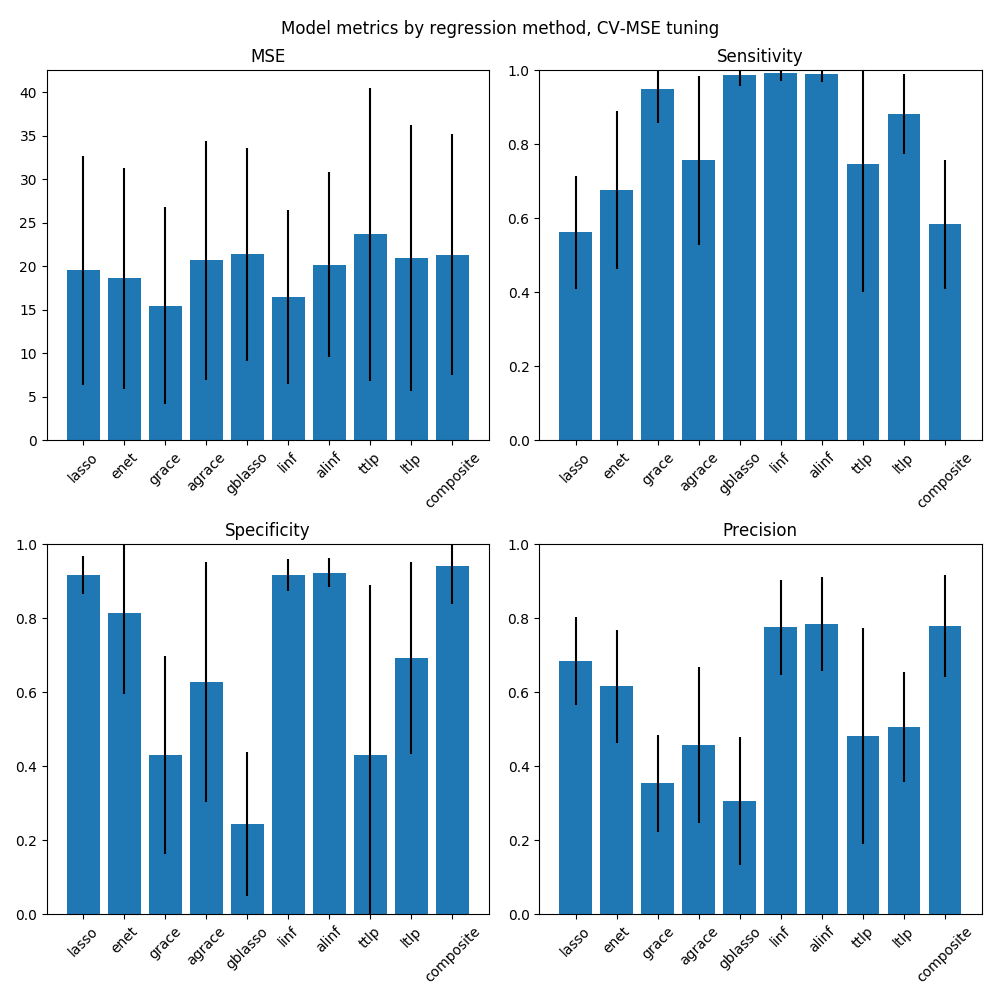
\includegraphics[scale=0.54]{cv_mse_tuning}
	\caption{CV-MSE tuning mean model metrics with standard deviation error bars for 20 synthetic datasets}
	\label{fig:met_cvmse}
\end{figure}

\section{Orchestrated tuning} \label{sec:disc_orc_tun}
The orchestrated hyperparameter tuning approach, discussed in Section \ref{sec:orc_par_tun}, was used to tune a subset of all regression methods. We excluded those approaches that inherently rely on previous estimates by other regression methods, namely the aGrace, aLinf, TTLP, LTLP and Composite. As a result, the ensemble of regression methods used for orchestrated tuning includes the Lasso, Elastic Net, Grace, GBLasso and Linf. Hyperparameter combinations selected by the CV-MSE tuning have been chosen for starting points in initialization of the orchestrated tuning procedure. The mean model metrics and their corresponding standard deviations for all synthetic datasets are shown on Table \ref{tab:met_orctun} and Figure \ref{fig:met_orchestrated}. All of the observations made in Section \ref{sec:disc_cvmse_tun} continue to be true for the results of this parameter tuning method. 

The GBLasso method continues to perform poor variable selection. However, in the context of orchestrated tuning its poor performance has a direct effect on the parameter tuning of all other methods in the ensemble. For some cases it might be suitable to discard such a method from the ensemble in order to avoid possible distortions in the tuning process. The discarded method can either be tuned separately or not considered at all in the experiments.

\begin{figure}[H]
	\centering
	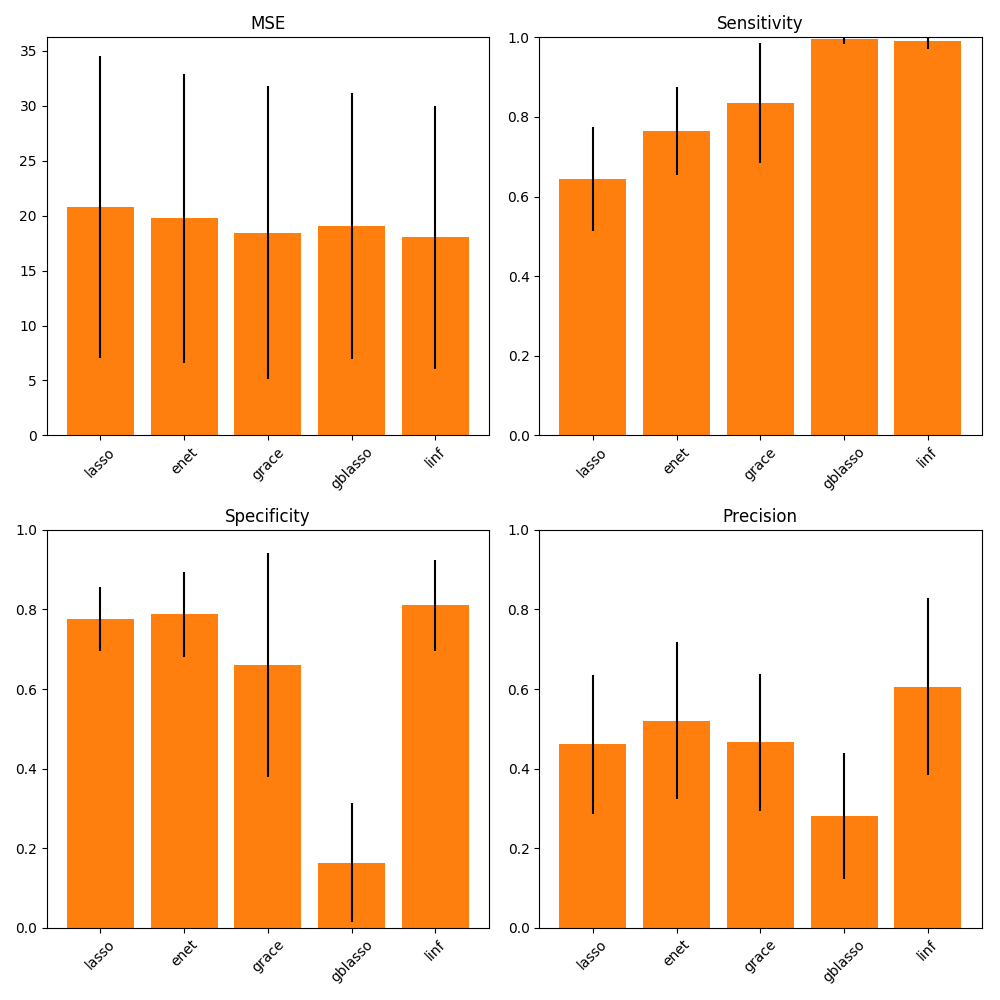
\includegraphics[scale=0.50]{orchestrated_tuning}
	\caption{Orchestrated tuning mean model metrics with standard deviation error bars for 20 synthetic datasets}
	\label{fig:met_orchestrated}
\end{figure}
\begin{table}[h!]
	\begin{center}
		\caption{Orchestrated tuning model metrics by regression method}
		\label{tab:met_orctun}
		\pgfplotstabletypeset[
		multicolumn names,
		col sep=comma,
		header=has colnames,
		columns={Method,MSE,Correlation,Sensitivity,Specificity,Precision},
		display columns/0/.style={string type, column type = {l}},
		display columns/1/.style={column type={S}, string type, column type = {c}},
		display columns/2/.style={column name=Correlation, column type={S}, string type, column type = {c}},
		display columns/3/.style={column name=Sensitivity, column type={S}, string type, column type = {c}},
		display columns/4/.style={column name=Specificity, column type={S}, string type, column type = {c}},
		display columns/5/.style={column name=Precision, column type={S}, string type, column type = {c}},
		every head row/.style={
			before row={\toprule}, 
			after row/.add={}{
				\arraybackslash
				&$(\sigma_{MSE})$&$(\sigma_{Correlation})$&($\sigma_{Sensitivity})$&$(\sigma_{Specificity})$&$(\sigma_{Precision})$\\
				\midrule\midrule
			}
		},
		every last row/.style={
			after row=\bottomrule
		},
		every nth row={2}{before row=\midrule},
		]{tables/metrics_orctun.csv}
	\end{center}
\end{table}

\section{Comparison of tuning approaches}
The model metrics results from Sections \ref{sec:disc_cvmse_tun} and \ref{sec:disc_orc_tun} have been merged for easier visual comparison of the different parameter tuning approaches. The combined results are shown in Table \ref{tab:met_comp} and Figure \ref{fig:met_comp}.

\begin{table}[H]
	\begin{center}
		\caption{Comparison of mean model metrics by parameter tuning method}
		\label{tab:met_comp}
		\pgfplotstabletypeset[
		multicolumn names,
		col sep=comma,
		header=has colnames,
		columns={Method,Tuning,MSE,Correlation,Sensitivity,Specificity,Precision},
		display columns/0/.style={string type, column type = {l}},
		display columns/1/.style={string type, column type = {l}},
		display columns/2/.style={column type={S}, string type, column type = {r}},
		display columns/3/.style={column name=Correlation, column type={S}, string type, column type = {r}},
		display columns/4/.style={column name=Sens, column type={S}, string type, column type = {r}},
		display columns/5/.style={column name=Spec, column type={S}, string type, column type = {r}},
		display columns/6/.style={column name=Prec, column type={S}, string type, column type = {r}},
		every head row/.style={
			before row={\toprule}, 
			after row={\midrule\midrule}
		},
		every last row/.style={
			after row=\bottomrule
		},
		every nth row={2}{before row=\midrule},
		]{tables/metrics_comparison.csv}
	\end{center}
\end{table}

The use of orchestrated tuning has improved certain model metrics for a subset of the regression methods, while the performance of other methods has been flawed. For example, the Specificity and Precision of the Grace method have been significantly improved at the cost of slightly reduced Sensitivity. Conversely, Sensitivity of the Lasso and Elastic Net has been increased at the expense of their Specificity and Precision. A number of factors could potentially affect the performance of the proposed orchestrated tuning approach:
\begin{itemize}
	\item The choice of alternative methods forming the orchestrated ensemble
	\item The hyperparameter search spaces selected for each ensemble method
	\item The starting points used to initialize the orchestrated tuning procedure
\end{itemize}

\begin{figure}[H]
	\centering
	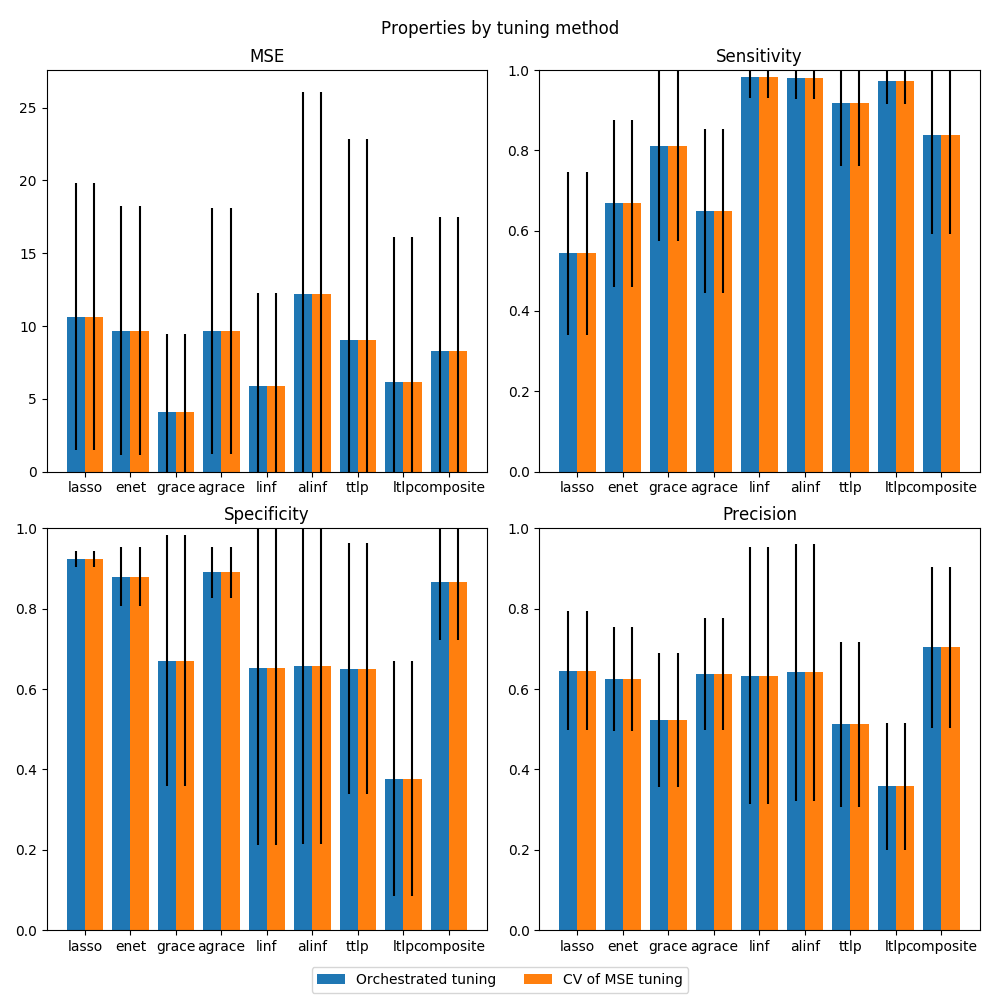
\includegraphics[scale=0.50]{tuning_method_comparison}
	\caption{Comparison of mean model metrics by parameter tuning method}
	\label{fig:met_comp}
\end{figure}

\section{Optimal hyperparameter value selection} \label{sec:opt_param_val}
Data about the optimal hyperparameter values selected when performing both kinds of parameter tuning on all synthetic datasets has been collected. It is used to select overall best combination of hyperparameter values for each regression method for use on a real dataset similar to the synthetic datasets.

\subsubsection{Lasso}
The distribution of tuning choices for the alpha hyperparameter is shown in Figure \ref{fig:tun_lasso}. Multiple values in the range $[0.05, 0.2]$ have been selected most times, of which $alpha = 0.1$ is chosen for use on the real dataset.
\begin{figure}[H]
	\centering
	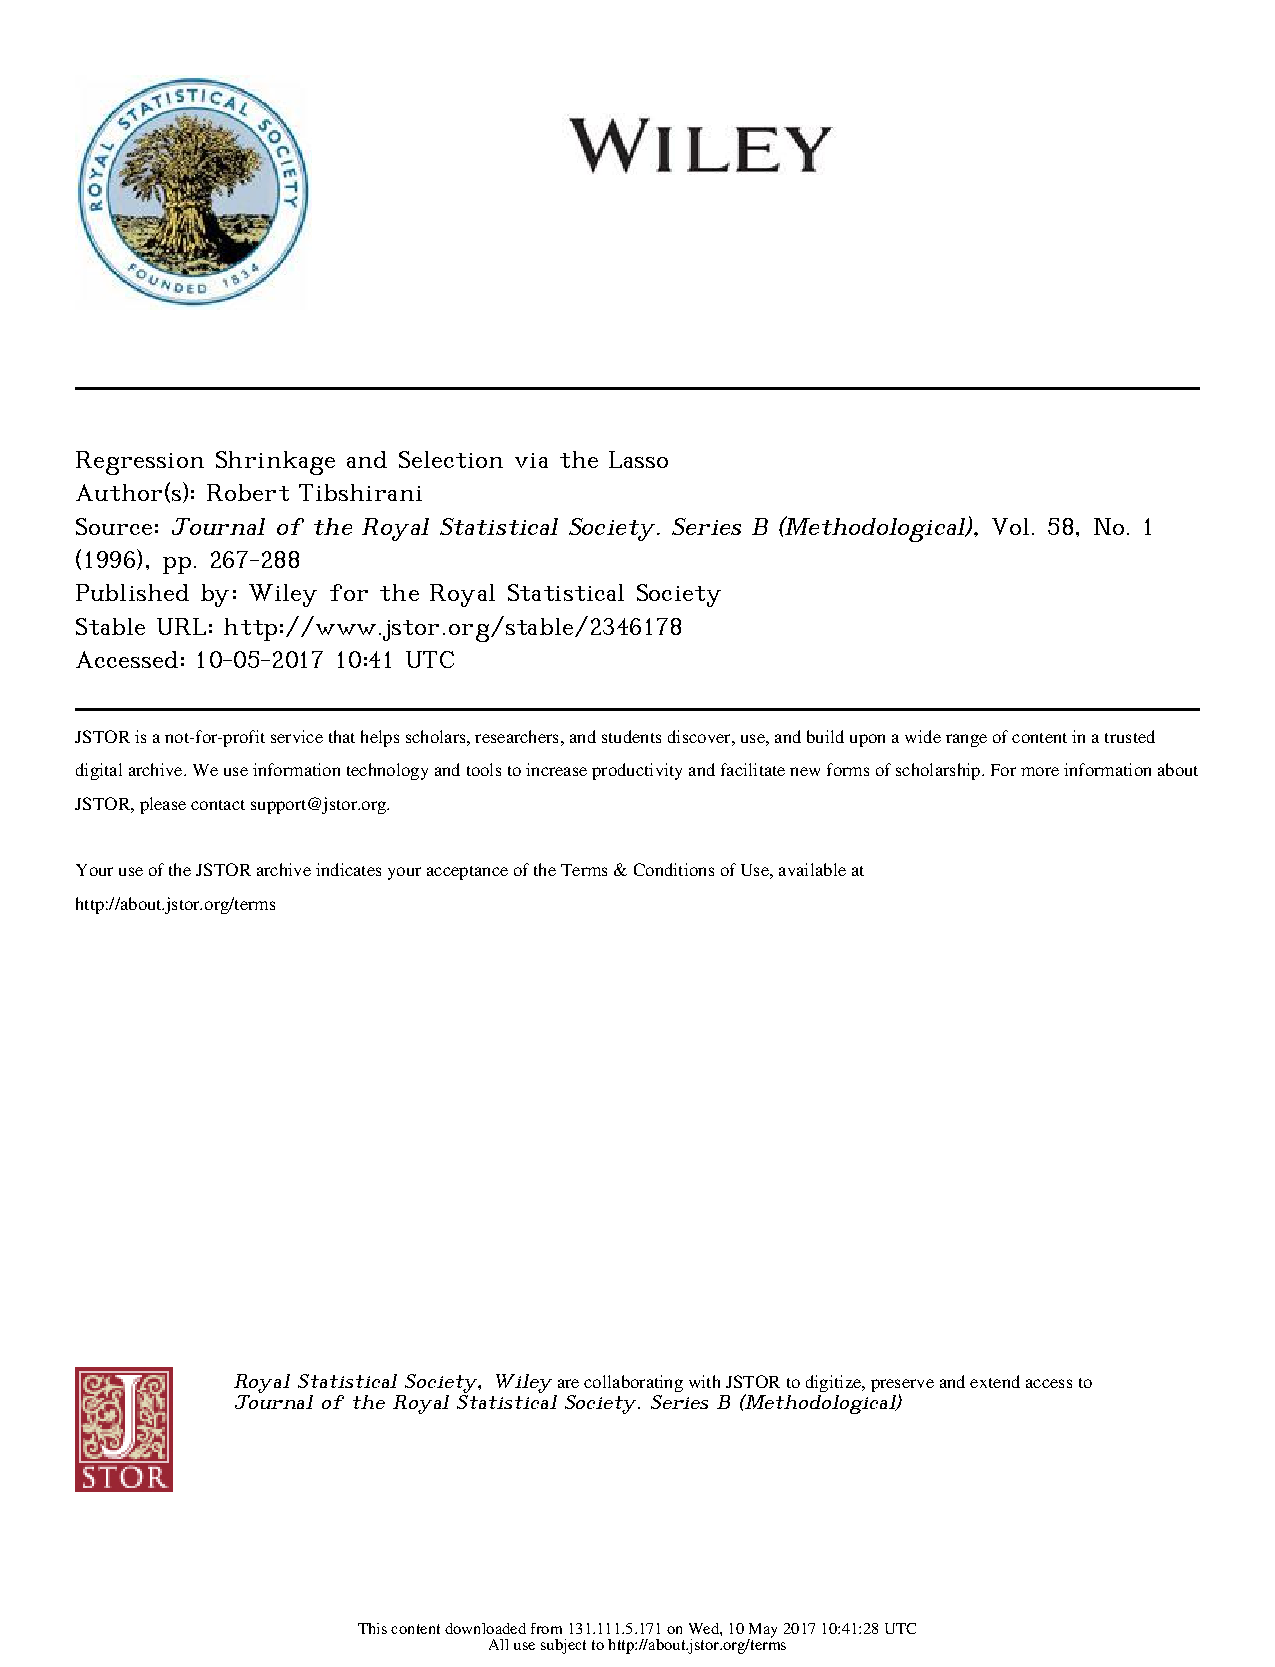
\includegraphics[scale=0.66]{tuning/lasso}
	\caption{Lasso distribution of selected parameter values}
	\label{fig:tun_lasso}
\end{figure}

\pagebreak

\subsubsection{Elastic Net}
The distribution of tuning choices for combinations of the alpha and L1 ratio hyperparameters is shown in Figure \ref{fig:tun_enet}. The evident choice of alpha value for use on the real dataset is $0.2$, but selected values for the L1 ratio parameter are more diversely spread. Although its most commonly selected value is 0.99, we choose a value of $L1\ ratio = 0.8$ for use on the real dataset in order to differentiate the behavior of Elastic Net from that of the pure Lasso.
\begin{figure}[H]
	\centering
	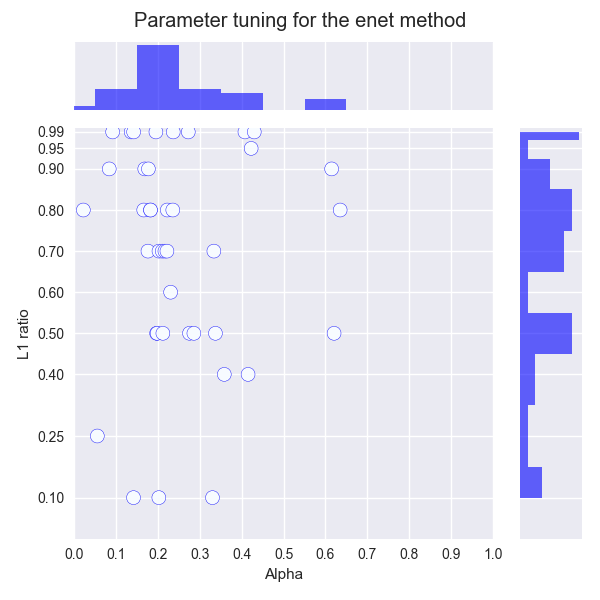
\includegraphics[scale=0.66]{tuning/enet}
	\caption{Elastic Net distribution of selected parameter combinations}
	\label{fig:tun_enet}
\end{figure}

\pagebreak

\subsubsection{Grace}
The distribution of tuning choices for combinations of the lambda 1 and lambda 2 hyperparameters is shown in Figure \ref{fig:tun_grace}. As the results suggest, the most commonly selected tuning parameter combination is $(\lambda_1=100,\lambda_2=10000)$ and it is chosen for use on the real dataset.
\begin{figure}[H]
	\centering
	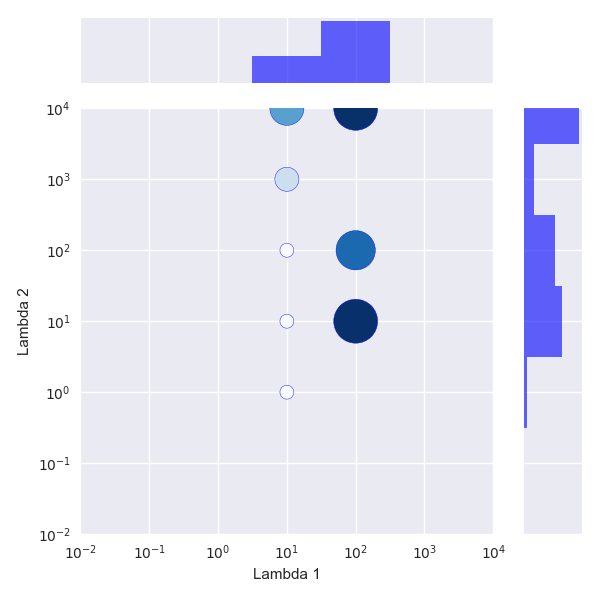
\includegraphics[scale=0.66]{tuning/grace}
	\caption{Grace distribution of selected parameter combinations; darker blue and larger marker size indicate a higher frequency of choice}
	\label{fig:tun_grace}
\end{figure}

\pagebreak

\subsubsection{aGrace}
The distribution of tuning choices for combinations of the lambda 1 and lambda 2 hyperparameters is shown in Figure \ref{fig:tun_agrace}. The tuning parameter combination $(\lambda_1=100,\lambda_2=0.01)$ is selected for the largest fraction of the synthetic datasets and therefore is chosen for use on the real dataset.
\begin{figure}[H]
	\centering
	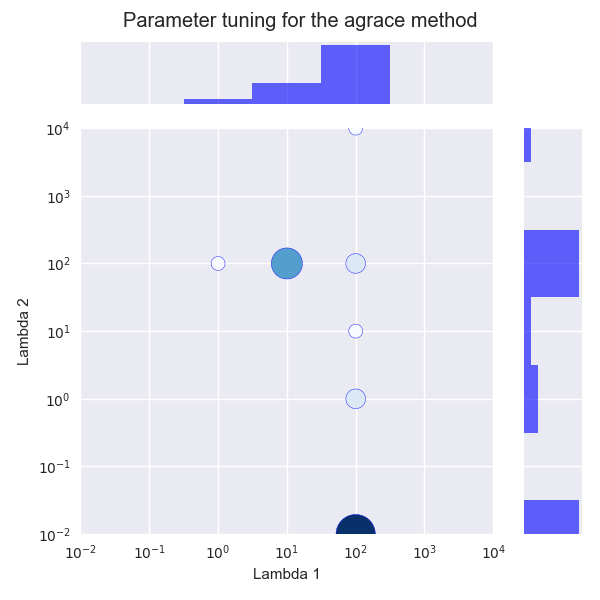
\includegraphics[scale=0.66]{tuning/agrace}
	\caption{aGrace distribution of selected parameter combinations; darker blue and larger marker size indicate a higher frequency of choice}
	\label{fig:tun_agrace}
\end{figure}

\pagebreak

\subsubsection{GBLasso}
The distribution of tuning choices for combinations of the gamma and lambda hyperparameters is shown in Figure \ref{fig:tun_gblasso}. The combination of parameter values selected most often is clearly $(\gamma = 4, \lambda=100)$ and it is chosen for use on the real dataset.
\begin{figure}[H]
	\centering
	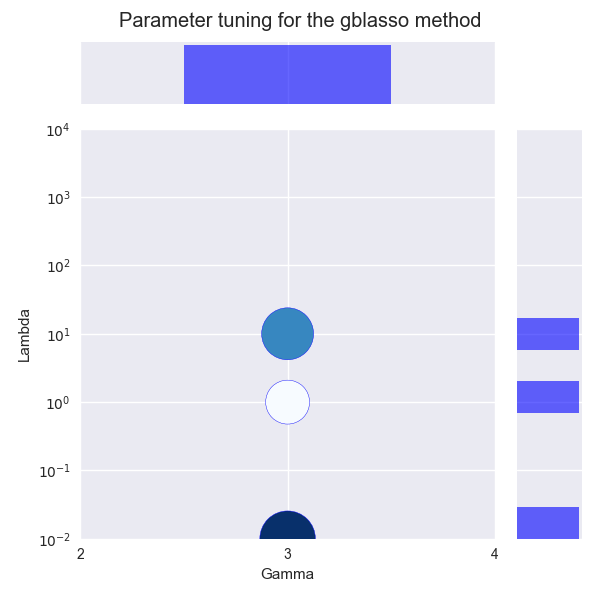
\includegraphics[scale=0.66]{tuning/gblasso}
	\caption{GBLasso distribution of selected parameter combinations; darker blue and larger marker size indicate a higher frequency of choice}
	\label{fig:tun_gblasso}
\end{figure}

\pagebreak

\subsubsection{Linf}
The distribution of tuning choices for the C hyperparameter is shown in Figure \ref{fig:tun_linf}. The value selected for most datasets is $C = 25$ and it is chosen for use on the real dataset.
\begin{figure}[H]
	\centering
	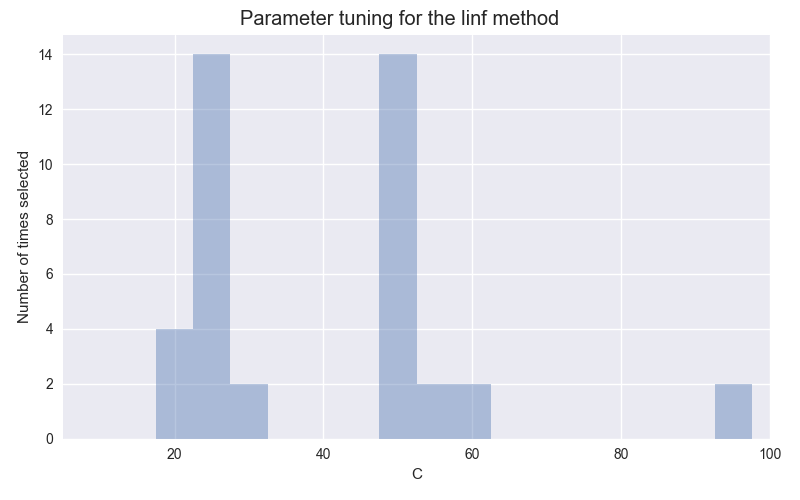
\includegraphics[scale=0.66]{tuning/linf}
	\caption{Linf distribution of selected parameter values}
	\label{fig:tun_linf}
\end{figure}

\pagebreak

\subsubsection{aLinf}
The distribution of tuning choices for the E hyperparameter is shown in Figure \ref{fig:tun_alinf}. The values selected most often are 25 and 35, of which $E = 25$ is chosen for use on the real dataset.
\begin{figure}[H]
	\centering
	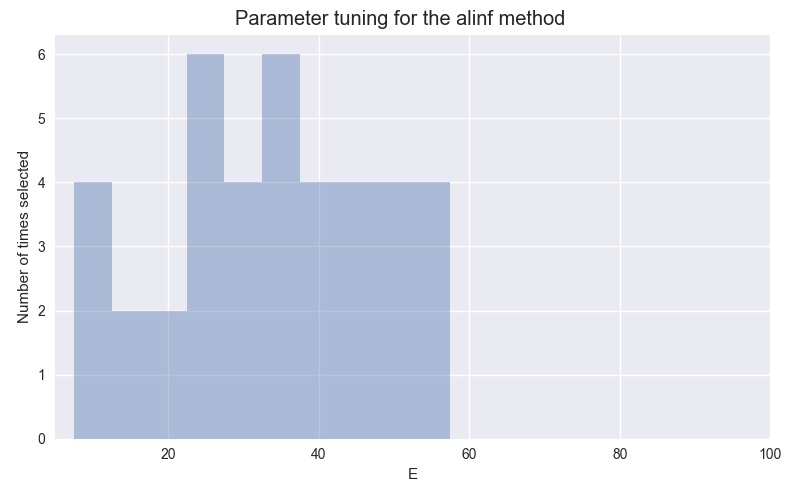
\includegraphics[scale=0.66]{tuning/alinf}
	\caption{aLinf distribution of selected parameter values}
	\label{fig:tun_alinf}
\end{figure}

\pagebreak

\subsubsection{TTLP and LTLP}
The TTLP and LTLP methods use search spaces for their tuning parameters derived from dataset properties and the Lasso estimate. For this reason attempting to extract an optimal combination of hyperparameter values from tuning with external independent datasets is not feasible. 

\subsubsection{Composite}
The distribution of tuning choices for the vote threshold hyperparameter is shown in Figure \ref{fig:tun_composite}. For most synthetic datasets a value of 0.9 is chosen. Because the methods in the ensemble are less than 10, in practice this means that all underlying regression methods need to have selected a given predictor for it to be selected by the composite method. The vote threshold value of 0.9 is chosen for use on the real dataset.
\begin{figure}[H]
	\centering
	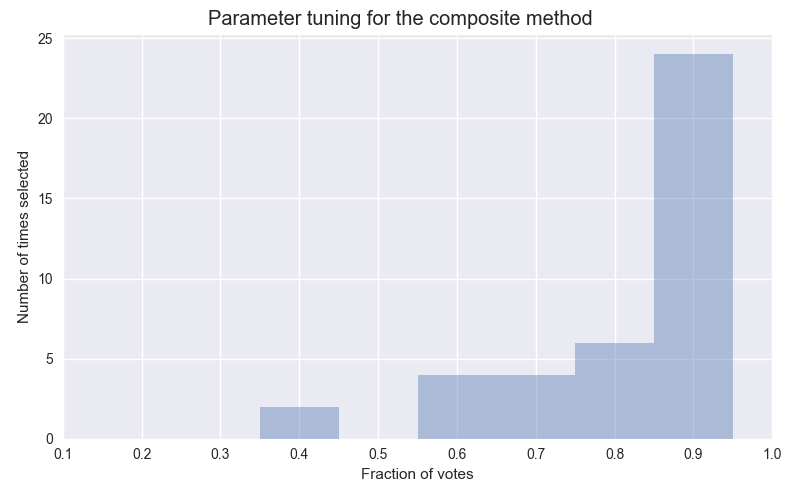
\includegraphics[scale=0.66]{tuning/composite}
	\caption{Composite method distribution of selected parameter values}
	\label{fig:tun_composite}
\end{figure}
